\documentclass[11pt,a4paper,titlepage, ngerman]{article}

\usepackage[utf8]{inputenc}	% Diese Pakete sind
\usepackage[T1]{fontenc}		% für die Verwendung 
\usepackage{ngerman}			% von Umlauten im tex-file
\usepackage{lmodern}			% Schriftart, die am Bildschirm besser lesbar ist
\usepackage{graphicx}			% Zum Einbinden von Formeln
\usepackage{url}					% Zur Darstellung von Webadressen
\usepackage{siunitx}
\usepackage{amsmath}			% für equation*
\usepackage{subcaption}
\usepackage{wrapfig}

\begin{document}
%	\setlength{\parindent}{0em} 
	
	\begin{titlepage}
		\centering
		{\scshape\LARGE Versuchsbericht zu \par}
		\vspace{1cm}
		{\scshape\huge E4 -- Kennlinien\par}
		\vspace{2.5cm}
		{\LARGE Gruppe 10 Mi\par}
		\vspace{0.5cm}
		{\large Alex Oster (E-Mail: a\_oste16@uni--muenster.de) \par}
		{\large Jonathan Sigrist (E-Mail: j\_sigr01@uni--muenster.de ) \par}
		\vfill
		durchgeführt am 8.11.2017\par
		betreut von\par
		{\large David \textsc{Pahl}}
		
		\vfill
		
		{\large \today\par}
	\end{titlepage}
		
	\tableofcontents
	
	\newpage
	
	\section{Kurzfassung}
		
		In diesem Bericht befassen wir uns mit Kennlinien. Eine Kennlinie ist die Kurve, die entsteht, wenn man die Spannung gegen den Strom aufträgt. Aus dem Ohm'schen Gesetz $U=RI$ bzw. $I = \frac{1}{R}U $ ergibt sich, dass diese durch den Widerstand dargestellt wird. 
		
		Wir betrachten im Folgenden zwei Versuchen, die uns verschiedenen Arten von Widerständen näher bringen sollen. 
		
		In dem ersten Versuch betrachten wir fünf verschiedene Arten von Widerständen. Eine einfache Diode, eine Zenerdiode, einen NTC-Widerstand, eine Glüh- und eine Glimmlampe. Wir messen hierbei den Strom in Abhängigkeit von der Spannung und werten die Ergebnisse aus. Dazu gehen wir auf die Funktionsweise von Halbleitern und Glimmlampen ein. 
		
		Die Abhängigkeit des Widerstands von der Temperatur wird dann in dem zweiten Versuch betrachtet.
		Hierzu erhitzen wir einen Kupferdraht in Öl, lassen ihn danach abkühlen und messen durchgehend seinen Widerstand mit Hilfe einer Wheatstone'schen Brücke. Unsere Ergebnisse für den Kupferdraht verknüpfen wir dann mit der allgemeinen elektrischen Leitfähigkeit von Metallen.

	\section{Versuch 1: Strom-Spannungs-Charakteristik}
		
		\subsection{Methoden} %Aufbau und wie/was gemessen wird
		
		In Abb. \ref{Schaltskizze1} ist der Versuchsaufbau skizziert. Dabei
		
		\begin{figure}
			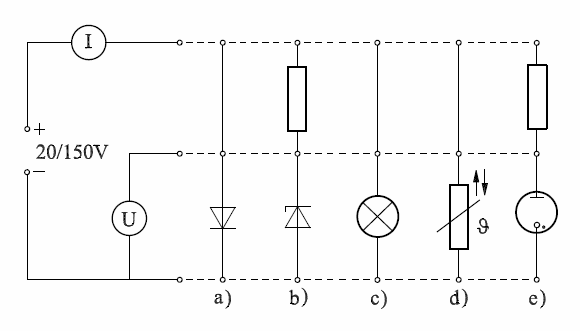
\includegraphics[width=\textwidth]{Versuch1.png}
			\caption{Schaltskizze zu Versuch 1}
			\label{Schaltskizze1}
		\end{figure}
		
		\subsection{Funktionsweise von Halbleitern}
		
		\subsection{a) Diode in Durchlassrichtung} %Erklärung Dioden, Messung und Schlussfolgerung

		\subsection{b) Zenerdiode} %Erklärung Zenerdioden, Messung und Schlussfolgerung
		
			\subsubsection{in Sperrrichtung}
			
			\subsubsection{in Durchlassrichtung}
			
		\subsection{c) Glühlampe} %Erklärung Glühlampe als Widerstand, Messung und Schlussfolgerung

		\subsection{d) NTC-Widerstand} %Erklärung NTC, Messung und Schlussfolgerung

		\subsection{e) Glimmlampe} %Erklärung Glimmlampe, Messung und Schlussfolgerung

	\section{Versuch 2: Widerstand in Abhängigkeit der Temperatur}		

		\subsection{Methoden} %Aufbau und wie/was gemessen wird
		
		\subsection{Messung}
		
		\subsection{Schlussfolgerung}		
	
	\newpage	
	\begin{thebibliography}	
		empty
	\end{thebibliography}	
			
\end{document} 